% !Mode:: "TeX:UTF-8" 

\BiChapter{克隆代码一致性维护需求预测实证研究}
{An Empirical Study on Clone Consistency-Requirement Prediction}


\BiSection{引言}
{Introduction}

%由于日益增长的软件开发的需求,开发人员在软件开发过程中通过复制粘贴既有代码,向系统中引入了大量克隆代码。
克隆代码在随着软件演化的过程中,可能会被程序开发人员修改而引发克隆代码的一致性问题。为解决此问题,本文在第三章和第四章分别在克隆代码创建时和变化时,对克隆代码的一致性维护需求进行了预测。但是,上述方法中仅考虑了贝叶斯网络方法,能否将其它机器学习方法(如支持向量机、决策树等)应用到此克隆需求预测中是一个值得研究的问题。此外,上述预测也没有和软件开发过程相结合,在开发过程中预测克隆一致性需求,可以切实的帮助程序开发人员避免克隆代码导致的额外维护代价和克隆一致性缺陷,从而帮助提高软件质量和可维护性。

鉴于此,在第三章和第四章研究的基础上,本章统一了克隆代码创建时和变化时的克隆代码一致性变化和维护需求定义,并使用五种不同的机器学习方法进行克隆一致性维护需求预测实证研究,并与软件开发过程相结合预测克隆一致性需求。首先通过构建软件系统的克隆家系来收集系统中所有的克隆实例(克隆创建实例和克隆变化实例),并提取不同的属性值表示不同的克隆实例。然后,使用五种不同的机器学习方法,分别在克隆创建时和变化时预测克隆代码的一致性维护需求。最后,结合软件开发过程,设计并实现了克隆代码一致性维护需求预测插件(CCRP),并可以嵌入到集成开发环境eclipse中预测克隆代码一致性需求。本章在四个开源软件系统上进行了实证研究,实验结果表明本文所提取的属性值可以适用于不同的机器学习方法上,且支持向量机方法更适合于克隆代码的一致性维护需求预测中。本章基于eclipse所实现的插件,可以帮助开发人员在软件开发过程中预测克隆代码的一致性,降低克隆代码导致的额外的维护代价,避免克隆变化导致的一致性缺陷,从而提高软件质量和可维护性。
%支持向量机方法具有最好的实验效果。



\BiSection{克隆代码一致性维护需求}
{Clone Consistency-Requirement}

\BiSubsection{研究问题}
{Research Problem}

在软件开发过程中,通过复制粘贴操作复用既有代码已经成为一种常见的软件开发手段,但是也会向软件系统中引入大量的克隆代码。这些新创建的克隆代码以及系统已经存在的克隆代码并不是静止不变的,会随着软件系统演化。在演化过程中,克隆片段片段可能会被软件开发员修改而发生变化,并可能进一步引发克隆组的一致性变化。克隆代码的一致性变化问题会影响软件质量和可维护性,原因在于:程序开发人员需要对发生变化的克隆进行一致性维护,会导致额外的一致性维护代价。而遗忘克隆的一致性变化,更会会导致克隆不一致缺陷,从而进一步增加软件的维护代价。

为了解决此问题,本文的第三章和第四章分别在克隆代码创建时和变化时,基于贝叶斯网络对克隆代码的一致性维护需求进行了预测,并取得了不错的预测效果。上述方法中仅仅使用了贝叶斯网络作为预测模型,但是在机器学习领域中仍然存在着其它的机器学习方法。因此,这启发了本章对克隆一致性预测的深入研究。首先,能否将克隆代码的一致性维护需求预测应用到其它的机器学习方法中。然后,在这些机器学习方法中,能否为开发人员确定一种通用的机器学习方法,可以同时应用于克隆创建时和克隆变化时的一致性需求预测中。 最后,对于两个不同的预测时刻(创建时和变化时),如何在软件开发过程帮助程序开发人员选择合适的预测时间,并达到最好的预测效果。更为重要的是,上述克隆一致性维护预测研究尚未与软件开发过程相结合,不能帮助程序开发人员在开发时预测克隆代码的一致性。

为了更好地帮助软件开发人员维护克隆代码,本章将结合其它机器学习方法和软件开发过程,对克隆代码进行一致性维护需求预测的实证研究。具体地,本章地研究问题如下:

{\bf Research Problem:} 克隆代码的一致性维护需求预测是否可以应用于其它的机器学习方法中,软件开发人员应如何结合软件开发过程中执行克隆一致性需求预测?\\
%{\em {\bf Research Problem:} Whether this clone consistency prediction task can be applied by other machine learning methods, and how should the developer determine perform such prediction in practice?}

为了解决本章的研究问题,将使用五种不同机器学习方法来预测克隆代码的一致性维护需求,并且分别在克隆代码创建时和克隆代码变化时进行预测。同时,在预测克隆一致性的过程中充分考虑并结合软件开发过程,比较和讨论两种不同预测的时间,从而帮助开发人员实际开发环境中执行克隆代码一致性预测,具体地,本文章研究问题可以细分为以下三个子问题,如下所示:

{\bf RQ1:}
%子问题1: 
在预测克隆代码创建时的一致性维护需求时,哪些机器学习方法可以用于该预测中,且所提取得度量值能否应用于其他的机器学习方法中,不同的机器学习方法预测效果是否一致,哪一种机器学习的方法能够取得最好的结果?
%%{\bf RQ1:} At clone creating time, which machine learning methods can be employed for clone consistency-requirement prediction?}\\
%在这个问题上,我们将会按照Wang等人的预测。与代码和上下文的属性集的变体。
%在这个子问题中,本章将第三章中的方法应用于其它的机器学习方法中,

{\bf RQ2:}
%子问题2: 
在预测克隆代码变化时的一致性维护需求时,哪些机器学习方法可以用于该预测中,且所提取得度量值能否应用于其他的机器学习方法中,不同的机器学习方法预测效果是否一致,哪一种机器学习的方法能够取得最好的结果?
%{\bf RQ2:} At clone changing time, which machine learning methods can be employed for clone consistency-requirement prediction?\\
%在这个问题上,我们将会按照Wang等人的预测。与代码和上下文的属性集的变体。
%在这个子问题中,本章将第第四章的方法应用于其它的机器学习方法中,

{\bf RQ3:}
%子问题 3: 
在实际开发过程中,程序开发人员应该如何结合软件开发过程选择合适的机器学习模型和预测时间,并对克隆代码进行一致性维护需求进行预测,从而都够达到最佳的预测效果?
%{\bf RQ3:} Which technique of machine learning should they employ as their preference? And, how the developers perform these clone predictions to achieve the preferably effectiveness in practice? 
}
%将对比两者并且,开发一个产假

鉴于此,本章基于不同的机器学习方法对克隆代码的一致性维护需求预测进行了一个实证研究,同时在克隆代码创建时和变化时预测克隆代码的一致性,并结合软件开发过程帮助程序开发人员选择合适和机器学习模型和预测时间已达到最佳的预测效果。首先,统一了克隆代码创建时和变化时的一致性变化及其一致性维护需求定义,可以在一个框架下预测克隆代码的一致性维护需求。然后,充分考虑了机器学习领域中五种不同的机器学习方法,并将其应用到克隆代码的一致性维护需求中。最后,本章结合软件开发过程,将克隆一致性维护预测方法嵌入到软件开发环境(eclipse)中,帮助程序开发人员实现边开发、边预测、边维护克隆代码,从而可以避免克隆一致性缺陷,并降低克隆代码的一致性维护代价。
%因此,本章方法可可以提高系统的可维护性和软件质量。
%\footnote{eclipse插件开发环境。}

\BiSubsection{克隆一致性维护需求定义}
{The Definitions for Clone Consistency-Requirement}

在克隆代码的整个演化周期中,克隆片段可能会被开发人员修改,从而导致克隆代码的一致性变化。在本文的第三章和第四章分别提供了两种不同形式的克隆代码一致性变化定义,从而适应于不同时间的克隆一致性维护需求预测中。本章将统一第三章和第四章的定义,以应用于本章地实证研究中。具体来说,克隆代码的一致性变化如下:\\

\begin{definition}
[一致性变化(Consistent Change)]  
\label{def-change}
给定两个克隆代码片段 $CF_1$和 $CF_2$,且它们被分别地修改为$CF'_1$和$CF'_2$。 如果对于一个非常小的阈值$\tau$,如果克隆代码$CF_1$和$CF_2$的变化满足以下条件,称此变化为{一致性变化(Consistent Change)} , 
  \[
  \begin{array}[t]{crl}
    \mathit{textSim}(CF_i, CF'_i) < 1 & \forall i \in \{1,2\} &(1) \\
    \multicolumn{2}{c}{| ~\mathit{textSim}(CF_1,CF'_1)  ~-~ \mathit{textSim}(CF_2,CF'_2) ~| ~< ~ \tau}  & (2)
  \end{array}
  \]
更具体地,如果克隆变化仅满足条件1,将其称为Type-1一致性变化({\em Type-1 Consistent Change});如果克隆变化同时满足条件1和条件2,将其称为Type-1一致性变化({\em Type-2 Consistent Change})。
\end{definition}

%\begin{definition}[{\bf Consistent Change}]  
%\label{}
%Given that two clone fragments $CF_1$, $CF_2$ are modified to $CF'_1$ and $CF'_2$ respectively. 
%We say this modification on $CF_1$ and $CF_2$ is a {\em\bf consistent change\/} if for some very small threshold $\tau$, 
%  \[
%  \begin{array}[t]{crl}
%    \mathit{textSim}(CF_i, CF'_i) < 1 & \forall i \in \{1,2\} &(1) \\
%    \multicolumn{2}{c}{| ~\mathit{textSim}(CF_1,CF'_1)  ~-~ \mathit{textSim}(CF_2,CF'_2) ~| ~< ~ \tau}  & (2)
 % \end{array}
 % \]
%More specifically, if they only satisfy condition 1, we call this as {\bf \em type-1 consistent change}, and if both conditions 1 and 2 are satisfied, we term it {\bf \em type-2 consistent change}.
%\end{definition}

定义中克隆代码$ CF_1 $和$ CF_2 $的变化情况由相似性度量$ \mathit {textSim} $进行定义,$textSim$与第三章和第四章计算方式相同。定义中的两个约束条件共同定义了克隆代码的一致性变化,约束条件$1$确保了克隆代码片段同时被修改,约束条件$2$克隆代码片段发生了一致性的变化,由变化阈值$\tau$指定。

其中,Type-1一致性变化又可以称为克隆创建时一致性变化,Type-2一致性变化又称为克隆变化时的一致性变化。这两种不同的一致性变化,将分别应用于两种不同时间的克隆一致性预测中。在克隆代码创建时,目标是避免新创建的克隆代码在其未来演化过程中的一致性变化,及其所导致额外的维护代价。所以,只要两个克隆片段同时变化,即认为会导致额外维护代价。因此,在克隆代码创建时使用使用Type-1一致性变化进行预测。在克隆代码变化时,目的是避免克隆变化可能导致的未来演化中的一致性变化,及其因此所引发的克隆一致性缺陷。所以, 不仅要求两个克隆代码片段同时变化,还需要发生相似的变化,否则将会引入克隆一致性缺陷,因此,在克隆代码变化时使用使用Type-2一致性变化进行预测。

在克隆演化过程中,克隆片段是以克隆组的形式出现在软件系统中。克隆代码的变化情况必然会导致克隆组的变化,而克隆组的变化使用克隆演化模式进行描述,即一致性变化模式。本文给出演化过程中克隆组的一致性变化模式定义,如下所示:\\


\begin{definition}
[一致性变化模式( Consistent Change Pattern)] 
\label{def-pattern}
在软件版本 $j+1$中存在一个克隆组$CG'$ ,假设克隆组内至少存在两个克隆代码片段$CF'_1$ 和 $CF'_2$可以与映射到上一版本$j$的克隆组$CG$中,且 $CG$中与之对应的克隆代码片段的 $(CF_1,CF_2)$被修改为$(CF'_1,CF'_2)$。如果克隆片段之间的变化( $(CF_1,CF_2)$变化至$(CF'_1,CF'_2)$满足克隆片段的“一致性变化(Consistent Change)”,则称克隆组$CG'$具有一致性变化模式(Consistent Change Pattern)。
\end{definition}

%\begin{definition}[{\bf Consistent Change Pattern}] 
%\label{}
%{\em
%A clone group $CG'$ in software version $j+1$ possesses {\em\bf type-1 or 2 consistent change pattern} if there exists a pair of clones $CF'_1,$ and $CF'_2$  in $CG'$ which are mappable to a pair of clones $CF_1$ and $CF_2$ in a clone group $CG$ in version $j$ such that modification of code pairs from $(CF_1,CF_2)$ to $(CF'_1,CF'_2)$ is a type-1 or 2 consistent change. 
%} 
%\end{definition}

其中“一致性变化”为Type-1或Type-2一致性变化,相应的克隆组变化模式则为Type-1和Type-2一致性变化模式。在相邻的两个软件版本中,克隆组一致性变化模式可以描述克隆演化中由于克隆片段变化所引发的克隆组的变化情况。

回顾本章地研究内容是要在两种不同的时刻预测克隆代码的一致性维护需求,结合第三章和第四章的克隆实例的定义,这里将统克隆创建实例和克隆变化实例为克隆代码实例,如下所示:\\

\begin{definition}
[克隆实例( Clone Instance)] 
\label{def-instance}
克隆创建实例:软件版本 $j$中的一个克隆组$CG$是克隆创建实例,如果该克隆组$CG$是其克隆家系$CGE$的根节点。
克隆变化实例:
软件版本 $j$中的一个克隆组$CG$是克隆变化实例,如果克隆组$CG$中至少两个克隆片段发生变化且版本$j+1$ 中至少存在一个克隆组$CG'$与之对应(在同一克隆家系$CGE$中)。 
克隆实例: 将克隆创建实例和克隆变化实例统称为克隆实例。
\end{definition}
%In the above definitions, we identify a $CG$ created by a creating operation (copy and paste) as a new $CGE$ root that begins its evolution. 

%\begin{definition}[{\bf Clone Instance}] 
%\label{}
%{\bf Clone Creating Instance:}
%{\em 
%A clone group $CG$ in version $j$ is {\bf clone creating instance} if $CG$ is a root node in the clone genealogy ($CGE$). 
%}
%~\\
%{\bf Clone Changing Instance:}
%{\em A clone group $CG$ in version $j$ is a {\bf clone changing instance} if at least one clone group $CG'$ in version $j+1$ which is connected to $CG$ in the clone genealogy was modified. 
%}
%~\\
%{\bf Clone Instance:}
%{\em We call clone creating and changing instance as {\bf clone instance}.
%}
%\end{definition}


克隆实例在演化过程中可能会引发的克隆一致性变化,如果不能确保克隆的一致性,将会导致导致额外的维护代价和一致性缺陷。具体来说,对于克隆创建实例,本文认为Type-1一致性变化及其演化模式在克隆演化过程中可能会导致额外的克隆维护代价。对于克隆变化实例,本文认为Type-2一致性变化及其演化模式在克隆演化过程可能会导致克隆一致性缺陷。因此,本章尝试在不同的时间预测克隆实例的一致性维护需求,以避免额外的克隆维护代价和一致性缺陷。本章结合第三章和第四章的克隆代码一致性维护需求的定义,将克隆创建时和变化时的一致性维护需求统一为克隆一致性维护需求定义,如下所示:\\

\begin{definition}
[克隆一致性维护需求(Clone Consistency-Requirement)] 
 \label{def-requirement}
给定版本 $j$中一个克隆实例,$CG$满足克隆一致性维护需求(Consistency-Requirement),如果在版本$k$中存在一个克隆实例 $CG'$($k>j$)满足以下条件: (1) 在$CG'$中至少存在两个克隆片段在其克隆家系$CGE$中可以映射到克隆实例 $CG$中, (2) $CG'$ 具有“一致性变化模式”(Consistent Change Pattern)。反之,假如克隆实例$CG$ 不满足克隆一致性维护需求条件,称该克隆实例不需要一致性维护(consistency-requirement free,或者consistency-free)。
\end{definition}

%\begin{definition}[{\bf Clone Consistency-Requirement}] 
 %\label{}
%{\em
%A clone instance $CG$ in software version $j$ satisfies {\bf consistency-requirement\/} condition if there is a clone group $CG'$ in software version $k$, with $k>j$, such that (1) there is at least a pair of clones in $CG'$ that is mappable in clone genealogy to a pair of clones in $CG$, and (2) $CG'$ possesses ``consistent change pattern''. When $CG$ does not satisfy consistency-requirement, we say that it is {\bf consistency-requirement free\/}, or simply {\em consistency-free\/} or {\em free} for short. %\\
%We employed the type-1 consistent change pattern for clone creating instance, and type-2 for changing instance.c
%}
%\end{definition}

其中,“一致性变化模式”为Type-1或Type-2一致性变化模式,相应的克隆一致性需求为Type-1和Type-2一致性维护需求。其中,Type-1克隆一致性维护需求可以用于预测克隆创建实例,Type-1克隆一致性维护需求可以用于预测克隆变化实例。

最终,克隆一致性维护需求预测任务可以转化为以下问题:
%{\bf Prediction Task:}
 给定一个克隆实例,克隆创建实例或者克隆变化实例,判断该克隆实例是否满足克隆一致性维护需求。
 
 更进一步,本文将克隆代码一致性维护需求预测问题转换成为一个分类问题,因而可以使用机器学习中的方法来解决此问题。在本文第三章和第四章的研究中,仅仅考虑了贝叶斯网络方法,为了更深入研究克隆代码的一致性预测问题,本文将会使用五种不同的机器学习方法在预测克隆实例的一致性维护需求。将在后文中详细介绍。


\BiSection{基于机器学习的克隆代码一致性需求预测框架}
{The Framework for Clone Consistency-Requirement base on Machine Learning}

为解决本章所提出的克隆一致性需求维护预测问题,本文首先给出了一个方法框架。基于机器学习的克隆代码一致性需求预测框架如图~\ref{framework5}~所示。方法可以划分为三个阶段,克隆实例收集阶段、克隆实例表示阶段和一致性维护需求预测阶段。收集阶段旨在收集系统中全部的克隆实例(包括创建实例和变化实例),可将其用于使用机器学习方法中来训练预测模型。由于实际的克隆实例无法直接应用于机器学习方法中,因此在表示步骤中将提取不同的属性值表示克隆实例,所提取的属性值将包含克隆实例的有意义的信息。接下来,在预测步骤,使用属性化的克隆实例构建和训练机器学习模型,并使用其预测克隆实例的克隆一致性维护需求。


\begin{figure}[htbp]
\centering
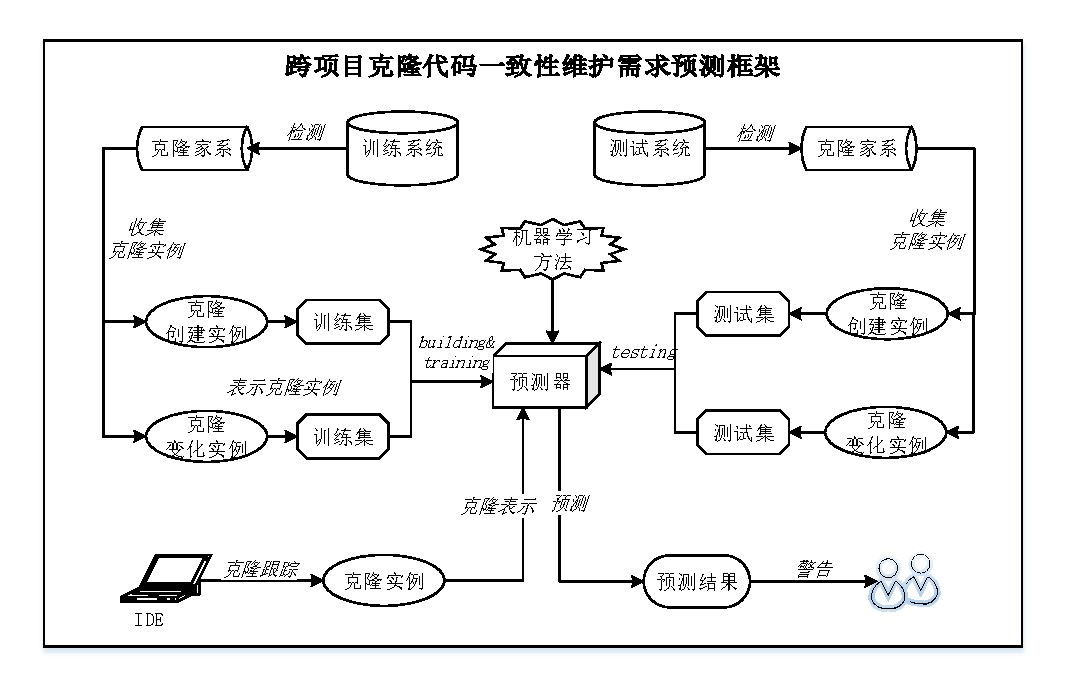
\includegraphics[width = 0.9\textwidth]{framework5.pdf}
\bicaption[framework5]{}{克隆代码一致性维护需求预测实证研究框架}
{Fig.$\!$}{The framework for empirical study on clone consistency prediction }
\vspace{-1em}
\end{figure}

具体来说,在收集阶段中,通过构建系统的克隆家系从软件中收集所有的克隆实例。使用NiCad来检测软件版本中的所有克隆,并通过在相邻版本的克隆组之间进行映射来构建克隆家系,用于识别克隆实例。在表示阶段中,通过提取属性值表示克隆创建和变化实例,提取代码属性和上下文属性表示克隆创建实例,提取代码属性、上下文属性和历史属性表示克隆变化实例。在预测阶段中,使用收集到的克隆创建实例训练贝叶斯网络,并在克隆创建时预测克隆一致性维护需求。在使用已构建好的模型进行预测时,可将该模型嵌入到软件开发环境中。软件开发环境需要实时监测克隆创建实例和变化实例并提取克隆实例的度量值。最后使用模型预测其一致性维护需求,根据预测结果提醒程序开发人员采取进一步的操作。

克隆实例有两种不同的预测结果,即满足一致性维护需求和不满足维护需求。
对于满足一致性维护需求实例来说,其在将来的演化中可能会引发一致性变化,程序开发人员需要采取相应的操作。例如,拒绝克隆创建实例或者检查克隆变化实例一致性。对于不满足一致性维护需求实例来说,其在将来的演化中不会引发一致性变化,程序开发人员需要采取相应的操作,如接受克隆创建实例。

本章使用多个不同的机器学习模型预测克隆实例的一致性。所提取的克隆实例的属性即为机器学习模型中的输入特征,用于构建不同机器模型的结构。所收集到的克隆变化实例可作为机器学习的训练集,用于训练机器学习模型的相关参数,细节可参考本文后续章节。
本章使用和比较五种不同的机器学习方法,以帮助开发人员选择最佳的预测手段。

\BiSection{克隆实例收集和表示}
{Collecting and Representing Clone Instance}

收集和表示克隆实例可以生成克隆一致性预测的训练集,为将克隆实例应用于机器学习中,提取不同的属性值表示克隆实例,从而可以训练机器学习模型。

\BiSubsection{克隆实例收集}
{Collecting Clone Instances}

收集克隆实例的目的在于生成克隆一致性预测的训练集,并将其用于训练机器学习模型。通过构建系统的克隆家系并识别其中的克隆演化模式,可以从软件中收集所有的克隆实例。首先使用NiCad来检测软件版本中的所有克隆,然后通过在相邻版本的克隆组之间进行映射来构建克隆家系,最后识别Type-1和Type-1克隆一致性演化模式识别系统中的克隆创建和变化实例。

根据定义~\ref{def-instance}~,克隆家系$CGE$中的初始节点即是克隆创建实例,发生变化的克隆组是变化实例,因此因此通过构建克隆家系可以收集克隆创建和变化实例。

(1)构建克隆家系。首先,下载系统所有版本的源代码,并使用NiCad的默认配置检测检测每一版本的中Type1-3的克隆代码。然后,通过映射所有相邻版本的克隆代码,构建系统中全部克隆家系。为完成版本间的映射,为每个克隆片段生成一个克隆区域描述符 $CRD$\cite{duala2010clone},使用基于$CRD$的克隆映射算法映射两个连续版本之间的所有克隆片段和克隆组\cite{ci2013new}\cite{ci2013newD}。根据克隆映射结果,构建系统的克隆家系。

(2)识别克隆演化模式和收集克隆实例。首先,识别克隆家系中的克隆演化模式,尤其是克隆一致性变化模式。构建克隆家系后,通过对比相邻版本的克隆代码,可以识别克隆家系的克隆演化模式(参考定义~\ref{def-evolutionpattern}~和\ref{def-pattern}~)。所识别的克隆演化模式有三个作用:(a)克隆演化模式可以帮助收集克隆变化实例。根据定义~\ref{def-evolutionpattern}~可以识别系统中发生一致性变化的克隆代码和克隆组,从而确定克隆家系中的克隆变化实例。(b)可以用于表示克隆变化实例,本文使用克隆演化模式作为表示克隆变化实例的部分演化属性。因此,克隆演化模式可以用于克隆变化实例表示中。(c)克隆演化模式可以帮助确认克隆一致性维护需求。根据定义~\ref{def-requirement}~,一致性维护需求,可以通过遍历克隆家系$CGE$是否发生了一致性变化模式进行确定。

然后,收集克隆实例。根据定义~\ref{def-instance}~通过遍历克隆家系的根节点,可收集系统中所有的克隆创建实例。在收集克隆变化实例后,还需确认该实例中的被复制和被粘贴代码(参见本文第三章收集克隆创建实例小节~\ref{lab-checkcopied}~)。根据定义~\ref{def-instance}通过识别克隆家系中的变化克隆组,便可以收集系统中的克隆变化实例。

(3)标识克隆变化实例的一致性维护需求。在收集所有的克隆实例后,还需确认相关实例的一致性维护需求。根据定义~\ref{def-requirement}~,通过遍历克隆实例所在的克隆家系$CGE$的演化情况确定其一致性维护需求。如果克隆实例在其演化过程中发生了一致性变化模式(~\ref{def-pattern}~),则该实例满足一致性维护需求,否则不满足维护需求。

\BiSubsection{克隆实例表示}
{Representing Clone Instance}

本章使用机器学习方法预测克隆代码的一致性维护需求,并使用软件中既有的克隆实例训练机器学习模型。但是,实际的克隆实例无法直接应用于机器学习中。因此,本文提取相应的属性值表示克隆代码实例,即提取代码、上下文两组属性代表克隆创建实例,提取代码属性、上下文属性和演化属性代表克隆变化实例。其中代码属性和上下文属性相似,但从不同的角度表示克隆创建实例和变化实例,克隆创建实例中的属性表示了创建时的被复制和被粘贴代码的特征,变化实例中的属性则表示了发生变化的克隆组的特征。

为表示克隆创建实例,对创建实例的被复制和粘贴克隆代码使用不同的属性。代码属性用于表示被复制的克隆的特征,包括:克隆代码粒度、Halstead属性、结构属性、参数访问数量、总函数调用次数、本地函数调用次数、库函数调用次数、其它调用次数。上下文属性用于表示被粘贴的克隆代码的特征,包括:代码相似度、局部克隆标识、文件名相似度、文件名相似度标识、方法名相似度、总参数名相似度、最大参数名相似度、总参数类型相似度、块信息标识。属性具体信息可以参考本文第二章相关属性值部分(~\ref{lab-creatingattribute}~)。

对于克隆变化实例,从克隆组的角度重新提取了代码属性和上下文属性,并从演化的角度新增演化属性。代码属性从代码自身的角度描述了克隆变化实例中克隆代码特征,包括克隆粒度、代码行平均、Halstead属性平均、结构属性平均、总函数调用次数平均、本地函数调用次数平均、库函数调用次数平均、其它调用次数平均。上下文属性描述了克隆变化实例所在的克隆组的克隆关系特征,包括代码相似度平均、文件名相似度平均、文件名相似度变量、方法名相似度平均、总参数名相似度平均、最大参数名相似度平均、总参数类型相似度平均、块信息标识。历史属性描述了克隆变化实例所在克隆组在克隆变化发生前的历史演化特征,包括变化实例寿命、历史演化模式统计、当前演化模式、历史变化统计。同时,还提供了克隆变化实例的变化属性。
属性具体信息可以参考本文第二章相关属性值部分(~\ref{lab-changingattribute}~)。


\BiSection{克隆一致性预测}
{Predicting Clone Consistency-Requirement}

本文将克隆代码的一致性维护需求问题,转化成了克隆创建实例和克隆变化实例的分类问题,即给定一个克隆实例,判别其是否满足克隆一致性维护需求。为了验证本文方法的有效性,本文使用了五种不同的机器学习方法,并将它们应用于克隆一致性维护需求的预测中。因此,本节先简单介绍所选择的机器学习方法。随后,使用属性化的克隆创建实例和克隆变化实例构建和训练不同的克隆一致性预测模型,并使用训练好的机器学习模型,在克隆代码创建时和变化时预测其一致性维护需求。

\BiSubsection{机器学习方法}
{The Employed Machine Learning Methods}
%{The Brief Introduction for Machine Learning Methods}

在本章的实证研究中,为解决本文所提出的研究问题,使用了五种不同的机器学习方法,即:{贝叶斯网络方法(Bayesian Network,简称为BayesNet)\cite{friedman1997bayesian}、朴素贝叶斯方法(Native Bayesian,本文简称为Native)\cite{john1995estimating},支持向量机方法(Support Vector Machine,简称为SVM)\cite{platt199912} 、K近邻方法(K-Nearest Neighbors,简称为KNN) \cite{aha1991instance}和决策树方法(Decision Tree,本文简称为Tree)\cite{quinlan2014c4}。

(1)贝叶斯网络方法\\
贝叶斯网络是一个是一种概率图型,使用已经观察到的事件来预测将来可能发生的事件\cite{friedman1997bayesian}。关于贝叶斯网络的信息可以参考本文第三章~\ref{lab-bayes}~节贝叶斯网络。

(2)朴素贝叶斯方法\\
朴素贝叶斯方法和贝叶斯网络类似,是运用贝叶斯定理为基础的简单概率分类器。但与贝叶斯网络不同的是,朴素贝叶斯方法的特征之间是强(朴素)独立的,因此称为朴素贝叶斯,即假定样本每个特征与其他特征都不相关。 

(3)支持向量机方法\\
支持向量机是另一种常见的机器学习方法,可以应用在分类与回归问题中。SVM模型将实例表示为空间中的点,并且试图构造一个超平面将不同类的实例(点)间隔开。更正式地来说,支持向量机在高维或无限维空间中构造超平面或超平面集合,可以用于分类问题中。直观来说,分类边界距离最近的训练数据点越远越好,因为这样可以缩小分类器的泛化误差。

以本文的克隆一致性需求分类为例,每一个克隆代码实例会抽象称为高维空间中的一个“点”,空间维数等同于所提取的属性数量。在使用SVM分类克隆实例时,将构造一个超平面分割开两种类别的克隆代码实例。

(4)K近邻方法\\
KNN方法是一种用于分类和回归的非参数统计方法。KNN是一种基于实例的学习方法,是局部近似和将所有计算推迟到分类之后的惰性学习。KNN会推迟对训练数据的建模,直到需要分类样本时才进行。在KNN分类中,输出是一个分类族群。一个实例的分类是由其邻居的“多数表决”确定的,K个最近邻居(k为正整数,通常较小)中最常见的分类决定了赋予该对象的类别。若k = 1,则该对象的类别直接由最近的一个节点赋予。邻居都取自一组已经正确分类(在回归的情况下,指属性值正确)的对象。

以本文克隆一致性预测为例,每一个克隆代码实例是KNN中的一个实例。在进行预测时,被预测的克隆实例的类别,将会有其最近的K个邻居进行表决,从而确定其一致性维护需求。

(5)决策树方法\\
机器学习中另一个常见的分类方法是决策树。决策树是一种简单但是广泛使用的分类器。通过训练数据构建决策树,可以高效的对未知的数据进行分类。决策树代表的是属性值与对象类别之间的一种映射关系。树中每个节点表示某个属性,而每个分叉路径则代表的某个可能的权重,而每个叶结点则对应从根节点到该叶节点所经历的路径所表示的对象的类别。决策树仅有单一输出,若欲有复数输出,可以建立独立的决策树以处理不同输出。

 以克隆一致性需求预测为例,克隆实例所提取的属性即是决策树中的属性,最后的克隆一致性维护需求则是对象的类别。
%决策树(decision tree)是一个树结构(可以是二叉树或非二叉树)。其每个非叶节点表示一个特征属性上的测试,每个分支代表这个特征属性在某个值域上的输出,而每个叶节点存放一个类别。使用决策树进行决策的过程就是从根节点开始,测试待分类项中相应的特征属性,并按照其值选择输出分支,直到到达叶子节点,将叶子节点存放的类别作为决策结果。

\BiSubsection{训练与预测}
{Training and Predicting}
%%%分成两个小节
%\BiSubsection{构建与训练预测器}
%{Building and Training Predictor}
%\BiSection{一致性预测}
%{Predicting Clone Consistency}

接下来,使用收集到的克隆实例训练不同的机器学习模型,并预测克隆代码的一致性维护需求。本章将在两个不同的时刻预测克隆代码的一致性维护需求,分别为为克隆创建时和克隆变化时,因此针对每一种机器学习方法,也会训练两种不同的模型。

本章没有对机器学习方法进行改进和研究,所使用模型的构建和训练通过调用现有机器学习工具包WEKA完成。本文使用WEKA 机器学习工具包内提供的机器学习算法进行一致性维护需求预测工作,通过实验对比上述五种机器学习算法的预测效果,从而帮助程序人员选择最好的机器学习模型。

对于每个软件系统,首先,通过收集系统中所有的克隆实例(创建实例和变化实例),并提取相应的属性,用于构建模型训练所需的数据集。然后,调用WEKA中的机器学习算法,分别构建克隆创建和变化时的预测器。对每一种机器学习方法,将会构建和训练两种模型一起预测克隆代码的一致性维护需求。

根据定义~\ref{def-requirement}~,克隆实例有两种不同的状态:需要一致性维护和不需要一致性维护。因此在进行一致性维护需求预测时,克隆实例也具有两种不同的预测结果:
\begin{itemize}
\item 
需要一致性维护:
若克隆创建实例的预测结果为“需要”,软件开发人员需要谨慎的执行克隆创建操作(复制和粘贴)。因为,该克隆创建实例,在未来演化的过程中可能会引发一致性变化,从而向系统中引入额外的维护代价。\\
若克隆变化实例的预测结果为“需要”,软件开发人员需要检测克隆变化实例所在的克隆组的一致性问题,考虑一致地修改组内其它的克隆代码。因为,该克隆变化实例,在未来演化的过程中可能会引发一致性变化,遗忘这种变化会向系统中引入缺陷,从而降低软件质量。
\item
不需要一致性维护:
若克隆创建实例的预测结果为“不需要”,软件开发人员可以自由的执行克隆创建操作(复制和粘贴),从而节约开发时间提高开发效率。因为,该克隆创建实例,在未来演化的过程中不会引发一致性变化,也不会导致额外的维护代价。\\
若克隆创建实例的预测结果为“不需要”,软件开发人员可以自由的修改克隆变化实例所在克隆组的克隆片段。因为,该克隆变化实例,在未来演化的过程中不会引发一致性变化,也不会导致一致性缺陷。
\end{itemize}


在使用已训练好的模型进行预测时,可以与软件开发过程相结合,将该模型嵌入到软件开发环境中,帮助程序开发人员实现边开发边预测克隆实例的一致性维护需求。首先,在软件开发环境中需监测程序员的复制粘贴操作和对克隆代码的修改,识别由此产生的克隆实例(克隆创建实例和变化实例)。然后,根据上文描述的代码、上下文和演化属性,提取相应的特征表示相应的克隆实例。最后,使用训练好的预测器预测相应克隆实例的一致性维护需求,根据预测结果提醒程序开发人员采取进一步的操作。



%%%当克隆克隆和更改实例发生时,我们打算为开发人员提供克隆一致性要求的这些预测因子。如图所示,这些预测变量可以集成到一个IDE中,如eclipse,可以帮助开发人员在开发阶段维护克隆的克隆和变化。这需要追踪克隆克隆和更改的其他要求,这可以由IDE支持。已经超出了我们的研究范围。当开发人员克隆或更改克隆片段时,已使用提取的属性生成克隆克隆或更改实例,并引用此实例。相关预测器将预测其一致性要求,并根据需要通知开发人员采取措施维护此代码克隆。



\BiSection{基于eclipse的克隆一致性维护需求预测插件}
{An eclipse Plug-in for Clone Consistency-Requirement Prediction}

为了与软件开发过程相结合,本章设计并实现了一个克隆代码的一致性维护需求插件,可以帮助开发人员预测克隆一致性维护需求。所设计的克隆一致性预测插件可以嵌入到软件开发环境中(eclipse),实现边开发、边预测、边维护克隆代码的一致性。基于eclipse的预测插件,可以帮助程序开发人员避免克隆变化导致的一致性维护代价及一致性缺陷,从而帮助提高软件质量和可维护性。

%本文所实现的eclipse插件可以帮助分析Jave语言程序,具有三个基本功能,

\BiSubsection{插件基本模块}
{Three Base Modules for Prediction Plug-in }

为了满足克隆代码的一致性需求预测,本文基于eclipse所设计的插件具有三个基本模块,可以帮助程序开发人员解析用java语言实现的软件系统。三个基本模块分别是:预处理模块、属性提取模块和一致性预测模块\footnote{本文插件目前仅支持基于java语言的源代码,但对于其它语言的扩展也较为容易。}。%预处理模块可以建克隆家系并识别克隆演化模式,从而帮助程序开发人员收集系统中的克隆实例。属性提取模块实现了对克隆实例的表示,可以提取不同的属性组表示相对应的克隆实例。一致性预测模块可以调用机器学习方法实现模型的训练,并预测克隆实例的一致性维护需求。

(1) 预处理模块。

预处理模块可以识别大多数克隆检测工具的结果,并构建克隆家系和识别克隆演化模式,从而实现对系统克隆实例的收集。
首先,需要人工的使用克克隆检测工具检测系统中的所有的克隆代码,并将检测结果作为插件的输入。 (本文中使用的克隆检测工具是NiCad \cite {roy2008clone})
对于软件系统的每一个版本,克隆代码将会被组成克隆组的形式,并使用文件名、起始行号表示所有的克隆代码,即“{\tt file \_name}”、“{\tt start \_line}”和“{\tt end \_line}”。然后,使用CRD重新描述克隆代码并重新组织为新的数据结构,从而方便构建克隆家系。最后,本插件将基于CRD对所有版本中的克隆代码,构建构建系统的克隆家系,并识别克隆演化模式。方法参加本文克隆家系构建和模式识别部分。
根据所构建的克隆家系和识别的演化模式,可以方便的获取系统中已经存在的克隆创建和变化实例。值得注意的是,构建克隆家系时需要系统所有版本的源代码,用于生成克隆代码的CRD表示。

(2) 属性提取模块

属性提取模块将不同的克隆代码实例抽象成相应的属性值,对克隆创建实例提取代码属性和上下文属性,对克隆变化实例提取代码属性、上下文属性、演化属性和变化情况。首先,代码属性和上下文属性提取,可以使用抽象语法树(Abstract Syntactic Tree,AST)对程序源代码进行解析获取。对每一个克隆代码以及克隆代码所在文件,使用Eclipse AST中的 ASTParser类将克隆片段所在源代码解析成AST\footnote{抽象语法树可参见:http://www.eclipse.org/articles/Article-JavaCodeManipulation\_AST/}。通过遍历语法树访问相应关键节点,根据本文描述的属性值计算克隆实例的代码属性和上下文属性。然后,历史属性提取,历史属性提取通过遍历克隆实例的克隆家系,根据属性描述计算相应历史属性。值得注意的是,属性提取时同样需要系统所有版本的源代码,用于生成克隆代码的抽象语法树和属性计算。%对克隆代码提取的工作可参见论文。\cite{yuan}


(3) 克隆一致性预测模块。

一致性预测模块实现了对相关机器学习模型的训练,并可以对在软件开发过程新产生的克隆创建实例和变化实例进行一致性维护需求预测。本插件并没有具体实现机器学习方法,而是通过调用WEKA中的API完成对机器学习模型的构造、训练和预测功能。WEKA是一个Java语言实现的数据挖掘和机器学习开源工具。WEKA提供了丰富的接口帮助程序开发人员调用相关的机器学习方法,可以使用极为灵活的方式对机器学习模型进行训练和预测\footnote{使用WEKA可参见:http://weka.wikispaces.com/。}。


\BiSubsection{克隆实例跟踪}
{Tracking Clone Instance in eclipse }

在软件开发过程中预测克隆代码的一致性需求维护,还需要实时的捕获软件中产生的克隆实例,即跟踪克隆实例的产生(克隆创建实例和克隆变化实例)。

(1)克隆创建实例跟踪

研究表明,软件中的克隆代码主要是由于复制和粘贴操作导致,即克隆创建实例产生的直接原因是程序开发人员的复制和粘贴操作。因此,测复制和粘贴操作即可跟踪克隆创建实例的产生。

%可以参考论文\cite{yuanD大论文}的实现

为在eclipse中监测程序开发人员的复制粘贴操作,


(2)克隆变化实例跟踪

为了跟踪克隆变化的产生,需要实现跟踪系统中克隆代码以及变化。


Tracking clones changes

\BiSubsection{克隆一致性预测插件使用}
{Three Base Modules for Prediction Plug-in }

由于机器学习模型的构建和训练往往需要大量的时间,不应该也不需要在每次开发时训练机器学习模型。因此,在实际的开发过程中,模型的训练和预测是分开进行的。
%因此,在使用一致性需求插件进行预测时,开发人员应该提前构建和训练好预测模型。

为了更为灵活的使用本文方法,提供两种构建和训练预测模型的方式。
第一个是用项目本身的历史数据来训练预测模型。在这种情况下,本文的插件首先调用预处理模块,构建项目本身所有克隆家系和收集项目中的所有克隆实例。然后调用属性提取模块,将提取收集到的克隆实例的属性值,并生成训练集。最后,使用该训练集建立和训练克隆一致性预测模型。
第二个其它项目数据作为训练集。原因在于,对于某些项目而言,由于实际版本的限制,其历史的克隆实例可能较少,不足以较好的训练所需要的模型。因此,需要使用其它项目的历史数据作为训练集。需要注意的是,随着时间的推移,当项目自身可以收集到足够的数据时,建议开发人员重新使用项目自身的数据训练机器学习模型,从而达到较好的预测效果。

当监测到具体的克隆实例产生时,调用已经训练好的机器学习模型进行预测。软件开发过程中,监测到克隆实例产生时,调用属性提取模块提取本次实例的属性,并使用训练好的一致性模型预测其一致性,根据预测结果通知程序开发人员采取相应措施。值得注意的是,在实际预测时,克隆变化实例预测需要项目的历史版本源代码,因为历史属性中包含克隆变化实例的历史变化过程。为了轻量化预测过程,程序开发人员可以将克隆变化实例中的历史变化属性移除。


\BiSection{实验结果与分析}
{Experiments Results and Analysis}

本节给出本章的实验结果与分析,首先简单介绍了实验所使用的实验系统和评估方法,然后详细给出每个实验的结果与分析。


\BiSubsection{实验系统与实验设置}
{Experimental Projects and Methodology}

为了解决本章的研究问题,本章在四个开源项目上进行了实验。表~\ref{clonesta}~给出了实验系统中克隆实例的统计信息,包括克隆创建实例和克隆变化实例。具体来说,表中第3、4列列出了不满足一致性维护需求的两类克隆实例的数量和比例。不需要一致性维护的克隆实例,在其未来的演化中不会导致一致性变化和额外的维护代价。需要一致性维护的克隆实例,在其演化过程中可能导致一致性变化及克隆一致性缺陷。

从表~\ref{clonesta}~中可以看出,系统中的克隆创建实例的数量是633到3666个,变化实例的数量为159到1040个。系统中克隆创建实例的数量要远于克隆变化实例的数量。其中,jEdit是四个系统中拥有克隆创建实例和克隆变化实例最少的。第二,软件系统中大部分的克隆创建实例在其演化过程中不满足一致性维护要求(比例从59.8\%到88.47\%)。这表明克隆操作已经成为开发人员的常用技术,并且大多数并不会在演化中引入一致的变化。第三,在克隆变化实例中,需要一致性维护的克隆实例比例占相当大的一部分,其比例为33\%到74 \%。尽管克隆变化实例的数量没有那么多,但是在系统中仍有几百个克隆变化实例,而这些变化似乎也更容易引发一致性变化,从而导致增加克隆代码一致性缺陷的风险。开发人员应该更加注意软件开发中的克隆变化。

\begin{table}[htbp]
\bicaption[clonesta]{}{实验系统的克隆实例信息统计}
{Table$\!$}{The statistics for clone instances in four projects}
\vspace{0.5em}
\centering
\wuhao
\begin{tabular}{ccccc}
\toprule[1.5pt]
~\multirow{2}{*}{类型}&\multirow{2}{*}{系统}&{不需要}&{需要} &\multirow{2}{*}{总数}\\
~&~&{一致性维护}&{一致性维护}&~\\
%~\multirow{2}{*}{\textbf{Instances}}&\multirow{2}{*}{\textbf{Project}}&\textbf{Consistency-} &\textbf{Meeting} &\multirow{2}{*}{\textbf{Total}}\\
%~&~&\textbf{Requirement Free}&\textbf{Consistency-Requirement}&~\\
\midrule[1pt]
\multirow{4}{*}{克隆创建实例}
&ArgoUML&	2574(77.07\%)&	766(22.93\%)&	3340\\
&jEdit&560(88.47\%)&	73(11.53\%)&	633\\
&jFreeChart&	2013(59.80\%)&	1353(40.20\%)&	3366\\
&Tuxguitar&	1016(71.10\%)&	413(28.90\%)&	1429\\
\hline
\multirow{4}{*}{克隆变化实例}
&ArgoUML&288(67.45\%)&139(32.55\%)&427\\
&jEdit&78(49.06\%)&81(50.94\%)&159\\
&jFreeChart&452(43.46\%)&588(56.54\%)&1040\\
&Tuxguitar&91(25.71\%)&263(74.29\%)&354\\
\bottomrule[1.5pt]
\end{tabular}
\end{table}

本章对克隆代码的一致性需求预测进行实证研究,目的是解决本文提出的研究问题:{克隆代码的一致性维护需求预测是否可以应用于其它的机器学习方法中,软件开发人员应如何结合软件开发过程中执行克隆一致性需求预测?}

本文将此研究问题划分为三个子问题,因此本章实验也相应的划分为三个部分以回答三个子问题。对于第一个研究问题,进行“创建时一致性预测实验”。对克隆创建实例进行实验,实验结果表明了五种不同机器学习方法的有效性。类似地,为了回答第二个研究问题,本章设计了“变化时一致性预测”实验。对克隆变化实例进行实验,也分析了五种不同的机器学习方法在克隆变化实例上的有效性。最后,第三个研究问题没有具体的实验,本章通过对比克隆创建实验和变化实验,并结合软件开发过程,回答本章提出的第三个研究问题。给出了一些相关的建议,帮助程序开发人员在开发实践中使用这些预测模型和技术。

在克隆创建实验和克隆变化实验中,与本文第三章和第四章相似,又分别进行了两种实验\footnote{值得注意的是,本章没有进行交叉验证实验。}:全属性实验和属性组实验,从两个不同的角度评估五种机器学习方法的有效性。全属性实验,使用所提取的全部属性进行预测,并对比五种机器学习方法。属性组实验中,使用不同的属性组进行实验,分析不同属性组的影响。

与第三章和第四章类似,克隆变化实例有两种类别,即需要一致性维护实例和不需要一致性维护实例。本章还从上述两个角度对本文方法进行了评估,进一步将实验划分为需要一致性维护实验和不需要一致性维护实验。“需要一致性维护实验”,分析了不同机器学习方法对满足一致性维护需求的实例的预测能力。与之相反,“不需要一致性实验”,分析了不同机器学习方法对不满足一致性维护需求的实例的预测能力。为了评测每一个实验结果,本文采用三个度量值评估预测效果,分别是:精确度(Precision)、召回率(Recall)和F值(F-measure)。其中在满足一致性的实验中。同时,为了给出给出更一般性的评估,并将两种克隆实例归并到一起,从而分析机器学习模型的一般化预测能力。采用平均精确度(Average Precision)、平均召回率(Average Recall)和平均F值(Average F-measure)。

这些满足维护需求的克隆实例,将导致未来的一致变化。当实例刚发生时,应该警告开发人员采取一定的措施。另一方面,不满足一致性需求的实例,将不会导致一致性变化,因此开发人员可以自由地自行复制或更改代码。


%我们的案例研究中,采用五种机器学习方法来探索这四个项目的这些预测的有效性。我们没有意图改进这些方法来适应这种一致性要求的预测。
%因此,我们使用包装WEKA来建立和训练我们所有需要的预测模型与不同的机器学习方法。WEKA是一种非常灵活且易于使用的数据挖掘工具,其中包含大量的分类/预测方法\cite{hall2009weka}。
%在本节中,我们将使用每种机器学习方法的缩写术语,贝叶斯网络为{\em BayesNet},本机贝叶斯为{\em Native},支持向量机为{\em SVM},K最近邻居作为{\em KNN}和设计树作为{\em 树}详细。

\BiSubsection{克隆创建时预测实验}
{Experiments for Clone Consistency-Requirement}

在本实验中,我们解决了克隆克隆实例的第一个子研究问题。
{\em {子问题1:}
在克隆克隆时间,其他机器学习方法是否可以用于克隆一致性要求预测?
属性集是否对此预测产生积极或消极的影响?}
我们采用五种不同的机器学习方法来预测这四个项目的克隆一致性,因此预测结果如表。

\begin{table}[htbp]
%%\caption{The Average Effectiveness of Creating Instances}
%%\label{creatingallavg}
\bicaption[creatingallavg]{}{不同机器学习方法的预测效果}
{Table$\!$}{The Average Effectiveness of Creating Instances}
\vspace{0.5em}
\centering
\wuhao
\begin{tabular}{cccccc}
\toprule[1.5pt]
{\textbf{Metric}}&{\textbf{Method}}&{\textbf{ArgoUML}}&{\textbf{jEdit}}&{\textbf{jFreeChart}}&{\textbf{Tuxguitar}}\\
\midrule[1pt]
\multirow{5}{*}{Percision}
&{BayesNet}&0.935&0.889&0.883&	0.831\\
&{Native}&	0.886&	0.871&	0.869&	0.793\\
&{SVM}&0.958&	0.924&0.906&0.888\\
&{KNN}&	0.94&0.886&0.9&	0.848\\
&{Tree}	&0.939&0.898	&0.893&0.889\\
\hline
\multirow{5}{*}{Recall}
&{BayesNet}& 0.936&	0.877&	0.882&	0.836\\
&{Native}&0.888&0.82&	0.868&0.794\\
&{SVM}& 0.958&0.921&0.904&0.883\\
&{KNN}&0.94&0.889&	0.9	&0.848\\
&{Tree}&0.94	&0.905&	0.892&0.891\\
\hline
\multirow{5}{*}{F-Measure}
&{BayesNet}&0.935&0.882&0.881&0.832\\
&{Native}&0.887&	0.84&0.867&0.794\\
&{SVM}&0.957&	0.903	&0.903&0.876\\
&{KNN}&0.94&0.887&	0.9	&	0.848\\
&{Tree}	&0.939&	0.901	&0.892&0.89\\
\bottomrule[1.5pt]
\end{tabular}
\end{table}

\begin{table}[htbp]
%%\caption{The Effectiveness of Creating Instances for free}
%%\label{creatingallfree}
%%\center
\bicaption[creatingallfree]{}{克隆创建实例的一致性自由的预测效果}
{Table$\!$}{The Effectiveness of Creating Instances for Consistency-Free}
\vspace{0.5em}
\centering
\wuhao
\begin{tabular}{cccccc}
\toprule[1.5pt]
{\textbf{Metric}}&{\textbf{Method}}&{\textbf{ArgoUML}}&{\textbf{jEdit}}&{\textbf{jFreeChart}}&{\textbf{Tuxguitar}}\\
\midrule[1pt]
\multirow{5}{*}{Percision}
&{BayesNet	}&0.945	&0.943	&0.879	&0.861\\
&{Natvie	}&0.917	&0.941	&0.863	&0.853\\
&{SVM}&	0.955	&0.919	&0.889	&0.872\\
&{KNN}&	0.96	&0.933	&0.905&	0.891\\
&{J48}&	0.953&	0.936	&0.891	&0.913\\
\hline
\multirow{5}{*}{Recall}
&{BayesNet}&	0.974&	0.916&	0.932	&0.917\\
&{Natvie	}&0.94&	0.85&	0.927	&0.858\\
&{SVM}&	0.992	&0.998	&0.959&	0.979\\
&{KNN}&	0.962&	0.943	&0.93	&0.896\\
&{J48}&	0.969&	0.959&	0.934&	0.935\\
\hline
\multirow{5}{*}{F-Measure}
&{BayesNet}&	0.959	&0.929&	0.905&	0.888\\
&{Natvie	}&0.928	&0.893	&0.894	&0.856\\
&{SVM}&	0.973	&0.957&	0.923	&0.923\\
&{KNN}&	0.961&	0.938	&0.917	&0.893\\
&{J48}&     0.961&	0.947	&0.912&	0.924\\
\bottomrule[1.5pt]
\end{tabular}
\end{table}

\begin{table}[htbp]
%%\caption{The Effectiveness of Creating Instances for Meeting Consistency-Requirement}
%%\label{creatingallmeeting}
\bicaption[creatingallmeeting]{}{符合研究生院绘图规范的表格}{Table$\!$}
{The Effectiveness of Creating Instances for  Meeting Consistency-Requirement}
\vspace{0.5em}
\wuhao
\centering
\begin{tabular}{cccccc}
\toprule[1.5pt]
{\textbf{Metric}}&{\textbf{Method}}&{\textbf{ArgoUML}}&{\textbf{jEdit}}&{\textbf{jFreeChart}}&{\textbf{Tuxguitar}}\\
\midrule[1pt]
\multirow{5}{*}{Percision}
&{BayesNet}&	0.808	&0.575	&0.809	&0.637\\
&{Natvie}&	0.714	&0.589	&0.78	&0.637\\
&{SVM}&	0.845	&0.329	&0.823	&0.646\\
&{KNN}&	0.864	&0.479	&0.854	&0.731\\
&{J48}&	0.841	&0.493	&0.831	&0.782\\
\hline
\multirow{5}{*}{Recall}
&{BayesNet}&	0.902	&0.472	&0.889	&0.758\\
&{Natvie}&	0.78	&0.339	&0.878	&0.646\\
&{SVM}&	0.969	&0.96	&0.931	&0.927\\
&{KNN}&	0.872	&0.522	&0.892	&0.74\\
&{J48}&	0.891	&0.61	&0.894	&0.83\\
\hline
\multirow{5}{*}{F-Measure}
&{BayesNet}&	0.853	&0.519	&0.847	&0.692\\
&{Natvie}&	0.746	&0.43	&0.826	&0.641\\
&{SVM}&	0.902	&0.49	&0.873	&0.762\\
&{KNN}&	0.902	&0.49	&0.873	&0.762\\
&{J48}&	0.865	&0.545	&0.861	&0.805\\
\bottomrule[1.5pt]
\end{tabular}
\end{table}




\begin{table*}[htbp]
%%\caption{The Average Effectiveness of Attribute Set for Creating Instances}
%%\label{csetavg}
\bicaption[creatingsetavg]{}{符合研究生院绘图规范的表格}{Table$\!$}
{The Average Effectiveness of Attribute Set for Creating Instances}
\vspace{0.5em}
\centering
\scriptsize
\begin{tabular}{cccccccccccccc}
\toprule[1.5pt]
\multirow{2}{*}{\textbf{Metric}}&\multirow{2}{*}{\textbf{Method}}&\multicolumn{3}{c}{\textbf{ArgoUML}}&\multicolumn{3}{c}{\textbf{jEdit}}&\multicolumn{3}{c}{\textbf{jFreeChart}}&\multicolumn{3}{c}{\textbf{Tuxguitar}}\\
\cline{3-14}
&&\textbf{All}&\textbf{Code}&\textbf{Context}&\textbf{All}&\textbf{Code}&\textbf{Context}&\textbf{All}&\textbf{Code}&\textbf{Context}&\textbf{All}&\textbf{Code}&\textbf{Context}~\\
\midrule[1pt]
\multirow{5}{*}{Percision}
&BayesNet&	0.935&	0.912&	0.917&		0.889&	0.885&	0.83&		0.883&	0.808&	0.903&		0.831&	0.811&	0.843\\
&Native&	0.886&	0.866&	0.877&		0.871&	0.865&	0.832&		0.869&	0.755&	0.873&		0.793&	0.747&	0.824\\
&SVM&	0.958&	0.928&	0.942&		0.924&	0.924&	0.909&		0.906&	0.819&	0.906&		0.888&	0.834&	0.873\\
&KNN&	0.94&	0.911&	0.933&		0.886&	0.903&	0.877&		0.9	&0.808&	0.898&		0.848&	0.806&	0.861\\
&Tree&	0.939&	0.904&	0.93&		0.898&	0.882&	0.876&		0.893&	0.802&	0.891&		0.889&	0.8&	0.881\\
\hline
\multirow{5}{*}{Recall}
&BayesNet&	0.936&	0.914&	0.919&		0.877&	0.869&	0.852&		0.882&	0.803&	0.903&		0.836&	0.817&	0.846\\
&Native&	0.888&	0.868&	0.88&		0.82&	0.836&	0.826&		0.868&	0.752&	0.873&		0.794&	0.756&	0.816\\
&SVM&	0.958&	0.929&	0.943&		0.921&	0.921&	0.918&		0.904&	0.806&	0.904&		0.883&	0.837&	0.874\\
&KNN&	0.94&	0.912&	0.934&		0.889&	0.912&	0.885&		0.9&	0.803&	0.898&		0.848&	0.81&	0.862\\
&Tree&	0.94&	0.905&	0.931&		0.905&	0.896&	0.889&		0.892&	0.796&	0.89&		0.891&	0.807&	0.882\\
\hline
\multirow{5}{*}{F-Measure}
&BayesNet&	0.935&	0.912&	0.917&		0.882&	0.876&	0.84&		0.881&	0.797&	0.902&		0.832&	0.811&	0.844\\
&Native&	0.887&	0.867&	0.878&		0.84&	0.848&	0.829&		0.867&	0.741&	0.872&		0.794&	0.75&	0.819\\
&SVM&	0.957&	0.927&	0.941&		0.903&	0.903&	0.907&		0.903&	0.797&	0.903&		0.876&	0.827&	0.869\\
&KNN&	0.94&	0.912&	0.933&		0.887&	0.905&	0.881&		0.9&	0.796&	0.897&		0.848&	0.807&	0.862\\
&Tree&	0.939&	0.904&	0.93&		0.901&	0.887&	0.881&		0.892&	0.788&	0.889&		0.89&	0.802&	0.881\\
\bottomrule[1.5pt]
\end{tabular}
\end{table*}


\begin{table*}[htbp]
\scriptsize
%%\caption{The Effectiveness of Attribute Set for Creating Instances for free}
%%\label{creatingsetfree}
\bicaption[creatingsetfree]{}{符合研究生院绘图规范的表格}{Table$\!$}
{The Effectiveness of Attribute Set for Creating Instances for Consistency-Requirement Free}
\vspace{0.5em}
\centering
\begin{tabular}{cccccccccccccc}
\toprule[1.5pt]
\multirow{2}{*}{\textbf{Metric}}&\multirow{2}{*}{\textbf{Method}}&\multicolumn{3}{c}{\textbf{ArgoUML}}&\multicolumn{3}{c}{\textbf{jEdit}}&\multicolumn{3}{c}{\textbf{jFreeChart}}&\multicolumn{3}{c}{\textbf{Tuxguitar}}\\
\cline{3-14}
&&\textbf{All}&\textbf{Code}&\textbf{Context}&\textbf{All}&\textbf{Code}&\textbf{Context}&\textbf{All}&\textbf{Code}&\textbf{Context}&\textbf{All}&\textbf{Code}&\textbf{Context}~\\
\midrule[1pt]
\multirow{5}{*}{Percision}
&BayesNet&0.945&	0.932	&0.929&		0.943&	0.942	&0.9	&	&0.879	&0.789	&0.898		&0.861	&0.848	0.88\\
&Native&0.917	&0.907&	0.913	&	0.941	&0.932&	0.906	&	0.863&	0.744&	0.873	&	0.853&	0.809	&0.89\\
&SVM&0.955&	0.937	&0.945	&	0.919	&0.919&	0.928&		0.889	&0.779&	0.889	&	0.872	&0.843	&0.877\\
&KNN&0.96	&0.94	&0.947	&	0.933&	0.934	&0.926	&	0.905&	0.787&	0.896	&	0.891&	0.856&	0.9\\
&Tree&0.953&	0.936	&0.943	&	0.936&	0.923	&0.921&		0.891&	0.778&	0.884	&	0.913	&0.842&	0.907\\

\hline
\multirow{5}{*}{Recall}
&BayesNet&0.974	&0.958	&0.969	&	0.916	&0.907&	0.936		&0.932	&0.916	&0.944	&	0.917	&0.905	&0.906\\
&Native&0.94	&0.924	&0.933&		0.85	&0.879&	0.896		&0.927&	0.892	&0.922	&	0.858	&0.86&	0.845\\
&SVM&0.992	&0.973&	0.983		&0.998	&0.998&	0.984		&0.959	&0.944	&0.959		&0.979	&0.947	&0.957\\
&KNN&0.962&	0.946&	0.969	&	0.943	&0.968&	0.945		&0.93&	0.919&	0.937	&	0.896	&0.881&	0.907\\
&Tree&0.969&	0.941	&0.969	&	0.959&	0.963	&0.957	&	0.934	&0.92&	0.939	&	0.935	&0.897	&0.93\\
\hline
\multirow{5}{*}{F-Measure}
&BayesNet&0.959&	0.945&	0.949	&	0.929	&0.924&	0.918	&	0.905&	0.848	&0.921	&	0.888&	0.875&	0.893\\
&Native&0.928&	0.915	&0.923	&0.893	&0.904	&0.901		&0.894&	0.811&	0.897	&	0.856	&0.834	&0.867\\
&SVM&0.973&	0.955&	0.964	&	0.957&	0.957&	0.955	&	0.923&	0.854	&0.923&		0.923&	0.892&	0.915\\
&KNN&0.961&	0.943&	0.958	&	0.938	&0.951&	0.935		&0.917	&0.848	&0.916&		0.893&	0.868	&0.903\\
&Tree&0.961&	0.938&	0.956	&	0.947	&0.942&	0.939	&	0.912&	0.843	&0.911&		0.924	&0.868&	0.918\\
\bottomrule[1.5pt]
\end{tabular}
\end{table*}


\begin{table*}[htbp]
\scriptsize
%%\caption{The Effectiveness of Attribute Set for Creating Instances for meeting}
%%\label{creatingsetmeeting}
\bicaption[sdfj1]{}{符合研究生院绘图规范的表格}{Table$\!$}
{The Effectiveness of Attribute Set for Creating Instances for Meeting Consistency-Requirement}
\vspace{0.5em}
\centering
\begin{tabular}{cccccccccccccc}
\toprule[1.5pt]
\multirow{2}{*}{\textbf{Metric}}&\multirow{2}{*}{\textbf{Method}}&\multicolumn{3}{c}{\textbf{ArgoUML}}&\multicolumn{3}{c}{\textbf{jEdit}}&\multicolumn{3}{c}{\textbf{jFreeChart}}&\multicolumn{3}{c}{\textbf{Tuxguitar}}\\
\cline{3-14}
&&\textbf{All}&\textbf{Code}&\textbf{Context}&\textbf{All}&\textbf{Code}&\textbf{Context}&\textbf{All}&\textbf{Code}&\textbf{Context}&\textbf{All}&\textbf{Code}&\textbf{Context}~\\
\midrule[1pt]
\multirow{5}{*}{Precision}
&BayesNet&	0.902	&0.844	&0.878	&	0.472	&0.447	&0.294	&	0.889	&0.836	&0.91	&	0.758	&0.719	&0.752\\
&Native&	0.78&	0.728&	0.756	&	0.339	&0.352	&0.266	&	0.878	&0.772	&0.873	&	0.646	&0.593	&0.662\\
&SVM&	0.969	&0.896	&0.934	&	0.96	&0.96&	0.769	&	0.931	&0.879	&0.931	&	0.927&	0.813	&0.863\\
&KNN&	0.872	&0.815	&0.888		&0.522	&0.66	&0.5		&0.892	&0.839	&0.9	&	0.74&	0.684	&0.767\\
&Tree&	0.891	&0.799&	0.885	&	0.61	&0.571	&0.529	&	0.894	&0.837&	0.901	&	0.83	&0.697	&0.817\\
\hline
\multirow{5}{*}{Recall}
&BayesNet&	0.808	&0.765&	0.752		&0.575	&0.575	&0.205	&	0.809&	0.636&	0.841	&	0.637&	0.6	&0.697\\
&Native&	0.714&	0.68	&0.701	&	0.589	&0.507&	0.288		&0.78	&0.542	&0.8	&	0.637	&0.501	&0.743\\
&SVM&	0.845&	0.779	&0.808	&	0.329	&0.329&	0.411	&	0.823	&0.601&	0.821	&	0.646	&0.567	&0.671\\
&KNN&	0.864&	0.798	&0.816	&	0.479	&0.479&	0.425	&	0.854&	0.63&	0.838		&0.731	&0.634&	0.751\\
&Tree&	0.841&	0.782	&0.803	&	0.493	&0.384&	0.37	&	0.831&	0.61&	0.817	&	0.782	&0.586	&0.765\\
\hline
\multirow{5}{*}{F-Measure}
&BayesNet&	0.853&	0.803&	0.81	&	0.519	&0.503&	0.242	&	0.847&	0.722&	0.874	&	0.692&	0.654&	0.724\\
&Native&	0.746&	0.703	&0.728		&0.43	&0.416	&0.276	&	0.826	&0.637	&0.835		&0.641	&0.543	&0.7\\
&SVM&	0.902&	0.834&	0.866&		0.49&	0.49	&0.536	&	0.873&	0.714	&0.873	&	0.762	&0.668&	0.755\\
&KNN&	0.868&	0.806&	0.85	&	0.5&	0.556	&0.459		&0.873	&0.72	&0.868		&0.736&	0.658	&0.759\\
&Tree&	0.865&	0.79&	0.842	&	0.545&	0.459&	0.435	&	0.861	&0.706&	0.857	&	0.805	&0.637&	0.79\\
\bottomrule[1.5pt]
\end{tabular}
\end{table*}

表{克拉克隆}表示克隆实例预测的有效性。从这个表可以看出,这种方法可以通过五种不同的机器学习方法{\ em有效地预测克隆一致性要求,从79.3\%到95.8\%的准确度从79.4\%回归到95.8\% ,F值从79.4\%至95.7\%。
比较所采用的学习方法的有效性,显然,{\em SVM}具有比这四个项目的其他方法更好的克隆预测能力。具体来说,SVM对于{\em ArgoUML,jEdit和jFreeChart}具有最好的结果,决策树具有最好的结果,SVM对于{\em Tuxguitar}来说是第二好的。与此同时,贝叶斯网络和本地贝叶斯方法在这四个项目中几乎保持了相对较差的预测结果。
因此,我们建议开发人员在需要预测克隆实例时首先考虑SVM。

为了探索属性集如何影响预测效果,我们仅使用一个属性集进行预测。属性集有效性的结果如表\ref{creatingset}所示。在这个表中,我们为所有属性集使用“全部”列,分别为其属性集使用“代码”,“上下文”。从这个表中可以看出,在不同属性的三个预测中,并没有显着差异。这表明我们的属性集不会对我们的预测产生负面影响。然而,对于这三个预测,我们还可以看到,在所有这四个项目的“属性”预测列(仅代码或上下文)中存在大部分相对较差的预测。具体来说,这三个项目的“代码”列{\em ArgoUML \/},{\em jFreeChart \/}和{\em Tuxguitar}对于这五个方法都有最差的结果,而“上下文” “{\em jEdit}”项目的列对于这五种方法几乎都是最差的.此外,我们将这些预测的结果与五种机器学习方法进行比较,我们得出的结论与SVM具有较好的预测能力相同。因此,建议在该预测中保留所有属性集,并首先优选SVM方法。


根据表\ref{克拉克隆}和表\ref{creatingset},我们可以给出我们对子问题1的建议。在克隆时间,五种机器学习方法可以应用于这种克隆预测,其结果非常相似。另外,他们之间还是有一点区别,SVM有更好的能力,我们建议开发选择这个来预测。同时,我们的属性集实验表明,所选择的属性对这一预测具有积极的影响,我们建议开发者可以自信选择它们进行预测。

\BiSubsection{2}
{2}
在本节中,我们解决克隆更改实例的第二个问题。{\em
{子问题2:}
在克隆更改时间,其他机器学习方法是否可以用于克隆一致性要求预测?
属性集是否对我们的预测产生积极或消极的影响?
}
为了解决这个问题,我们采用了五种不同的机器学习方法进行克隆更改的一致性,结果如表。
\begin{table}[htbp]
%%\caption{The Average Effectiveness of Changing Instances}
%%\label{changingallavg}
\bicaption[changingallavg]{}{符合研究生院绘图规范的表格}
{Table$\!$}{The Average Effectiveness of Changing Instances}
\centering
\wuhao
\begin{tabular}{cccccc}
\toprule[1.5pt]
{\textbf{Project}}&{\textbf{Metric}}&{\textbf{ArgoUML}}&{\textbf{jEdit}}&{\textbf{jFreeChart}}&{\textbf{Tuxguitar}}\\
\midrule[1pt]
\multirow{5}{*}{Percision}
&{BayesNet}&0.724&	0.686&	0.791&0.72\\
&{Native}& 0.734&	0.696	&0.778&	0.729\\
&{SVM}&0.744	&0.704&0.793	&0.733\\
&{KNN}&0.733	&0.597&	0.772&	0.672\\
&{Tree}&0.682	&0.581	&0.742	&0.637\\
\hline
\multirow{5}{*}{Recall}
&{BayesNet}&0.735	&	0.686&0.791&0.746\\
&{Native}&0.726&	0.692&0.778&0.737\\
&{SVM}&0.752	&0.704&0.791&0.734\\
&{KNN}&0.731	&	0.597	&	0.77	&	0.706\\
&{Tree}&0.698&	0.579	&	0.742&0.672\\
\hline
\multirow{5}{*}{F-Measure}
&{BayesNet}&	0.726	&	0.686	&0.79	&0.726\\
&{Native}&0.729&	0.689&0.778&0.733\\
&{SVM}&0.729&0.704	&0.789&	0.733\\
&{KNN}&0.732	&0.597	&0.771	&	0.683\\
&{Tree}&0.632	&	0.573&	0.739&0.651\\
\bottomrule[1.5pt]
\end{tabular}
\end{table}


\begin{table}[htbp]
%%\scriptsize
%%\caption{The Effectiveness of Changing Instances for Consistency-Requirement Free}
%%\label{changingallfree}
\bicaption[changingallfree]{}{符合研究生院绘图规范的表格}
{Table$\!$}{The Effectiveness of Changing Instances for Consistency-Requirement Free}
\vspace{0.5em}
\centering
\wuhao
\begin{tabular}{cccccc}
\toprule[1.5pt]
{\textbf{Project}}&{\textbf{Metric}}&{\textbf{ArgoUML}}&{\textbf{jEdit}}&{\textbf{jFreeChart}}&{\textbf{Tuxguitar}}\\
\midrule[1pt]
\multirow{5}{*}{Precision}
&{BayesNet}&0.774	&0.679	&0.783	&0.508\\
&{Native}&0.813	&0.723	&0.743	&0.488\\
&{SVM}&0.761	&0.707&	0.804&	0.483\\
&{KNN}&0.806&	0.592	&0.726&	0.39\\
&{Tree}&0.703	&0.59	&0.742&	0.302\\
\hline
\multirow{5}{*}{Recall}			
&{BayesNet}&0.858	&0.679&	0.719&	0.33\\
&{Native}&0.771	&0.603	&0.748	&0.44\\
&{SVM}&0.92&	0.679&	0.688	&0.473\\
&{KNN}&0.792&	0.577	&0.757	&0.253\\
&{Tree}&0.955&	0.462	&0.624	&0.209\\
\hline
\multirow{5}{*}{F-Measure}
&{BayesNet}&0.814	&0.679	&0.75	&0.4\\
&{Native}&0.791	&0.657&	0.745&	0.462\\
&{SVM}&0.833	&0.693	&0.741	&0.478\\
&{KNN}&0.799&	0.584	&0.741	&0.307\\
&{Tree}&0.81	&0.518	&0.678&	0.247\\
\bottomrule[1.5pt]
\end{tabular}
\end{table}

\begin{table}[htbp]
%%\scriptsize
%%\caption{The Effectiveness of Changing Instances for meeting}
%%\label{changingallmeeting}
\bicaption[changingallmeeting]{}{符合研究生院绘图规范的表格}
{Table$\!$}{The Effectiveness of Changing Instances for Meeting Consistency-Requirement }
\vspace{0.5em}
\centering
\wuhao
\begin{tabular}{cccccc}
\toprule[1.5pt]
{\textbf{Project}}&{\textbf{Metric}}&{\textbf{ArgoUML}}&{\textbf{jEdit}}&{\textbf{jFreeChart}}&{\textbf{Tuxguitar}}\\
\midrule[1pt]
\multirow{5}{*}{Precision}
&{BayesNet}&0.62	&0.691&	0.797	&0.793\\
&{Native}&0.571	&0.67	&0.805	&0.813\\
&{SVM}&0.709&	0.702	&0.784	&0.819\\
&{KNN}&0.583	&0.602	&0.807	&0.769\\
&{Tree}&0.639&	0.571&	0.742&	0.753\\
\hline
\multirow{5}{*}{Recall}
&{BayesNet}&0.482&	0.691&	0.847&	0.89\\
&{Native}&0.633&	0.778&	0.801&	0.84\\
&{SVM}&0.403&	0.728&	0.871&	0.825\\
&{KNN}&0.604&	0.617	&0.781&	0.863\\
&{Tree}&0.165	&0.691&	0.833&	0.833\\
\hline
\multirow{5}{*}{F-Measure}
&{BayesNet}&0.543	&0.691	&0.821	&0.839\\
&{Native}&0.601&	0.72&	0.803	&0.826\\
&{SVM}&0.514&	0.715	&0.825&	0.822\\
&{KNN}&0.594	&0.61	&0.793	&0.814\\
&{Tree}&0.263&	0.626&	0.785&	0.791\\
\bottomrule[1.5pt]
\end{tabular}
\end{table}



\begin{table*}[htbp]
\scriptsize
%%\caption{The Average Effectiveness of Attribute Set for Changing Instances}
%%\label{changingsetavg}
\bicaption[changingsetavg]{}{符合研究生院绘图规范的表格}
{Table$\!$}{The Average Effectiveness of Attribute Set for Changing Instances}
\vspace{0.5em}
\centering
\begin{tabular}{cccccccccccccccccc}
\toprule[1.5pt]
\multirow{2}{*}{\textbf{Metric}}&\multirow{2}{*}{\textbf{Method}}&\multicolumn{4}{c}{\textbf{ArgoUML}}&\multicolumn{4}{c}{\textbf{jEdit}}&\multicolumn{4}{c}{\textbf{jFreeChart}}&\multicolumn{4}{c}{\textbf{Tuxguitar}}\\
\cline{3-18}
%%&&\textbf{All}&\textbf{Code}&\textbf{Context}&\textbf{Evolution}&\textbf{All}&\textbf{Code}&\textbf{Context}&\textbf{Evolution}&\textbf{All}&\textbf{Code}&\textbf{Context}&\textbf{Evolution}&\textbf{All}&\textbf{Code}&\textbf{Context}&\textbf{Evolution}~\\
&&\textbf{All}&\textbf{Code}&\textbf{Cont}&\textbf{Evo}&\textbf{All}&\textbf{Code}&\textbf{Cont}&\textbf{Evo}&\textbf{All}&\textbf{Code}&\textbf{Cont}&\textbf{Evo}&\textbf{All}&\textbf{Code}&\textbf{Con}&\textbf{Evo}~\\
\midrule[1pt]
\multirow{5}{*}{Percision}
&BayesNet&	0.724&	0.737&	0.712&	0.727&		0.686&	0.698&	0.673&	0.654&	0.791&	0.76&	0.773&	0.76&		0.72&	0.686&	0.672&	0.727\\
&Native&	0.734&	0.743&	0.693&	0.723&		0.696&	0.662&	0.636&	0.676&	0.778&	0.756&	0.731&	0.747&		0.729&	0.7	&0.69&	0.719\\
&SVM&	0.744&	0.737&	0.736&	0.758&		0.704&	0.749&	0.687&	0.642&		0.793&	0.742&	0.769&	0.775&		0.733&	0.678&	0.726&	0.699\\
&KNN&	0.733&	0.692&	0.688&	0.725&		0.597&	0.522&	0.617&	0.68&		0.772&	0.703&	0.744&	0.741&		0.672&	0.639&	0.659&	0.669\\
&Tree&	0.682&	0.689&	0.713&	0.696&		0.581&	0.579&	0.571&	0.595&		0.742&	0.746&	0.711&	0.733&		0.637&	0.621&	0.658&	0.634\\
\hline
\multirow{5}{*}{Recall}
&BayesNet&	0.735&	0.742&	0.724&	0.733&		0.686&	0.698&	0.673&	0.654&	0.791&	0.761&	0.774&	0.761&		0.746&	0.718&	0.709&	0.743\\
&Native&	0.726&	0.738&	0.681&	0.71&		0.692&	0.66&	0.635&	0.673&		0.778&	0.757&	0.732&	0.742&		0.737&	0.703&	0.686&	0.737\\
&SVM&	0.752&	0.742&	0.74&	0.766&		0.704&	0.748&	0.686&	0.642&		0.791&	0.739&	0.768&	0.775&		0.734&	0.678&	0.718&	0.698\\
&KNN&	0.731&	0.698&	0.689&	0.733&		0.597&	0.522&	0.616&	0.679&		0.77&	0.7	&0.742&	0.738&		0.706&	0.681&	0.689&	0.689\\
&Tree&	0.698&	0.7	&0.726&	0.703&		0.579&	0.579&	0.553&	0.591&		0.742&	0.745&	0.711&	0.734&		0.672&	0.653&	0.672&	0.678\\
\hline
\multirow{5}{*}{F-Measure}
&BayesNet&	0.726&	0.739&	0.715&	0.729&		0.686&	0.698&	0.673&	0.654&		0.79&	0.76&	0.772&	0.76&		0.726&	0.695&	0.683&	0.732\\
&Native&	0.729&	0.74&	0.686&	0.714&		0.689&	0.659&	0.634&	0.671&		0.778&	0.756&	0.731&	0.743&		0.733&	0.702&	0.688&	0.725\\
&SVM&	0.729&	0.712&	0.707&	0.75&	0.704&	0.748&	0.684&	0.642&		0.789&	0.733	&0.765&	0.773&		0.733&	0.678&	0.721&	0.698\\
&KNN&	0.732&	0.694&	0.688&	0.727&		0.597&	0.522&	0.616&	0.678&		0.771&	0.701&	0.743&	0.739&		0.683&	0.655&	0.671&	0.677\\
&Tree&	0.632&	0.634&	0.694&	0.635&		0.573&	0.577&	0.533&	0.584&		0.739&	0.741&	0.711&	0.731&		0.651&	0.635&	0.664&	0.651\\
\bottomrule[1.5pt]
\end{tabular}
\end{table*}

\begin{table*}[htbp]
\scriptsize
%%\caption{The Effectiveness of Attribute Set for Changing Instances for free}
%%\label{changingsetfree}
\bicaption[changingsetfree]{}{符合研究生院绘图规范的表格}
{Table$\!$}{The Effectiveness of Attribute Set for Changing Instances for Consistency-Requirement Free}
\vspace{0.5em}
\centering
\begin{tabular}{cccccccccccccccccc}
\toprule[1.5pt]
\multirow{2}{*}{\textbf{Metric}}&\multirow{2}{*}{\textbf{Method}}&\multicolumn{4}{c}{\textbf{ArgoUML}}&\multicolumn{4}{c}{\textbf{jEdit}}&\multicolumn{4}{c}{\textbf{jFreeChart}}&\multicolumn{4}{c}{\textbf{Tuxguitar}}\\
\cline{3-18}
%%&&\textbf{All}&\textbf{Code}&\textbf{Context}&\textbf{Evolution}&\textbf{All}&\textbf{Code}&\textbf{Context}&\textbf{Evolution}&\textbf{All}&\textbf{Code}&\textbf{Context}&\textbf{Evolution}&\textbf{All}&\textbf{Code}&\textbf{Context}&\textbf{Evolution}~\\
&&\textbf{All}&\textbf{Code}&\textbf{Cont}&\textbf{Evo}&\textbf{All}&\textbf{Code}&\textbf{Cont}&\textbf{Evo}&\textbf{All}&\textbf{Code}&\textbf{Cont}&\textbf{Evo}&\textbf{All}&\textbf{Code}&\textbf{Con}&\textbf{Evo}~\\
\midrule[1pt]
\multirow{5}{*}{Precision}
&BayesNet&0.774&	0.795	&0.769	&0.788		&0.679	&0.703	&0.667	&0.653		&0.783	&0.731	&0.764	&0.739	&	0.508	&0.424	&0.393	&0.5\\
&Native&0.813	&0.817	&0.781&	0.808	&	0.723	&0.676	&0.643	&0.697	&	0.743	&0.726&	0.698&	0.685	&	0.488	&0.42	&0.394	&0.486\\
&SVM&	0.761	&0.747	&0.744	&0.78	&	0.707	&0.732	&0.7	&0.633		&0.804	&0.759	&0.775	&0.77	&	0.483&	0.374	&0.455	&0.413\\
&KNN&	0.806	&0.766	&0.768	&0.782	&	0.592	&0.513	&0.602	&0.69		&0.726	&0.644	&0.697	&0.688		&0.39	&0.31	&0.354	&0.37\\
&Tree&	0.703&	0.704	&0.738	&0.705	&	0.59	&0.58&	0.531	&0.61		&0.742	&0.749	&0.666	&0.724		&0.302	&0.265	&0.342	&0.298\\
\hline
\multirow{5}{*}{Recall}
&BayesNet&0.858&	0.833	&0.844	&0.826	&	0.679&	0.667	&0.667	&0.628	&	0.719	&0.71	&0.695	&0.695&		0.33	&0.275	&0.242&	0.396\\
&Native&0.771	&0.788	&0.733	&0.747	&	0.603&	0.59&	0.577	&0.59	&	0.748	&0.708	&0.675	&0.752	&	0.44	&0.407	&0.407&	0.374\\
&SVM&	0.92	&0.934&	0.938&	0.91	&	0.679	&0.769	&0.628	&0.641&		0.688&	0.586	&0.657	&0.688	&	0.473	&0.374	&0.495	&0.418\\
&KNN&	0.792	&0.795	&0.771	&0.837		&0.577	&0.526	&0.641	&0.628		&0.757	&0.692	&0.721	&0.73	&	0.253	&0.198	&0.253	&0.297\\
&Tree&	0.955	&0.958	&0.92&	0.962		&0.462	&0.513	&0.769&	0.462&		0.624&	0.622&	0.67&	0.626&		0.209&	0.198&	0.297&	0.187\\
\hline
\multirow{5}{*}{F-Measure}
&BayesNet&0.814&	0.814	&0.805&	0.807	&	0.679&	0.684	&0.667	&0.641	&	0.75	&0.721&	0.728	&0.716	&	0.4	&0.333&	0.299	&0.442\\
&Native&0.791&	0.802&	0.756&	0.776		&0.657	&0.63&	0.608	&0.639	&	0.745	&0.717	&0.686	&0.717	&	0.462&	0.413	&0.4	&0.422\\
&SVM&	0.833	&0.83&	0.829&	0.84&		0.693&	0.75&	0.662&	0.637&		0.741&	0.662&	0.711&	0.727&		0.478&	0.374&	0.474	&0.415\\
&KNN&	0.799	&0.78	&0.769&	0.809&		0.584	&0.519	&0.621	&0.658	&	0.741	&0.667	&0.709	&0.708	&	0.307	&0.242	&0.295	&0.329\\
&Tree&	0.81	&0.812	&0.819&	0.814&		0.518&	0.544&	0.628&	0.526&		0.678&	0.68&	0.668	&0.671&		0.247&	0.226&	0.318&	0.23\\
\bottomrule[1.5pt]
\end{tabular}
\end{table*}

\begin{table*}[htbp]
\scriptsize
%%\caption{The Effectiveness of Attribute Set for Changing Instances for meeting}
%%\label{changingsetmeeting}
\bicaption[changingsetmeeting]{}{符合研究生院绘图规范的表格}
{Table$\!$}{The Effectiveness of Attribute Set for Changing Instances for Meeting Consistency-Requirement}
\vspace{0.5em}
\centering
\begin{tabular}{cccccccccccccccccc}
\toprule[1.5pt]
\multirow{2}{*}{\textbf{Metric}}&\multirow{2}{*}{\textbf{Method}}&\multicolumn{4}{c}{\textbf{ArgoUML}}&\multicolumn{4}{c}{\textbf{jEdit}}&\multicolumn{4}{c}{\textbf{jFreeChart}}&\multicolumn{4}{c}{\textbf{Tuxguitar}}\\
\cline{3-18}
%%&&\textbf{All}&\textbf{Code}&\textbf{Context}&\textbf{Evolution}&\textbf{All}&\textbf{Code}&\textbf{Context}&\textbf{Evolution}&\textbf{All}&\textbf{Code}&\textbf{Context}&\textbf{Evolution}&\textbf{All}&\textbf{Code}&\textbf{Context}&\textbf{Evolution}~\\
&&\textbf{All}&\textbf{Code}&\textbf{Cont}&\textbf{Evo}&\textbf{All}&\textbf{Code}&\textbf{Cont}&\textbf{Evo}&\textbf{All}&\textbf{Code}&\textbf{Cont}&\textbf{Evo}&\textbf{All}&\textbf{Code}&\textbf{Con}&\textbf{Evo}~\\
\midrule[1pt]
\multirow{5}{*}{Precision}
&BayesNet&0.62	&0.616&	0.595&	0.6&		0.691&	0.694	&0.679	&0.655	&	0.797	&0.782	&0.781	&0.776		&0.793	&0.776	&0.768&	0.805\\
&Native&0.571	&0.591&	0.51&	0.547	&	0.67&	0.648	&0.629	&0.656	&	0.805	&0.78	&0.756	&0.794	&	0.813	&0.797	&0.792&	0.799\\
&SVM&	0.709	&0.716	&0.719	&0.714		&0.702	&0.766	&0.674	&0.65		&0.784	&0.729	&0.764	&0.778	&	0.819	&0.783	&0.82&	0.798\\
&KNN&	0.583	&0.539	&0.522	&0.605		&0.602	&0.532	&0.632	&0.67		&0.807	&0.749	&0.78	&0.782		&0.769	&0.753	&0.765	&0.772\\
&Tree&	0.639	&0.657	&0.662	&0.676		&0.571	&0.578	&0.609	&0.58		&0.742	&0.743	&0.745&	0.74		&0.753	&0.745	&0.767	&0.751\\
\hline
\multirow{5}{*}{Recall}
&BayesNet&0.482	&0.554	&0.475	&0.54		&0.691	&0.728	&0.679	&0.679		&0.847	&0.799	&0.835	&0.811		&0.89	&0.871	&0.871	&0.863\\
&Native&0.633	&0.633	&0.576	&0.633		&0.778	&0.728	&0.691	&0.753		&0.801	&0.794	&0.776	&0.735		&0.84	&0.806	&0.783	&0.863\\
&SVM&	0.403	&0.345	&0.331	&0.468		&0.728	&0.728	&0.741	&0.642		&0.871	&0.857	&0.854	&0.842		&0.825	&0.783	&0.795	&0.795\\
&KNN&	0.604	&0.496	&0.518	&0.518		&0.617	&0.519	&0.593	&0.728		&0.781	&0.706	&0.759	&0.745		&0.863	&0.848	&0.84	&0.825\\
&Tree&	0.165	&0.165	&0.324	&0.165		&0.691	&0.642	&0.346	&0.716		&0.833	&0.84	&0.741	&0.816		&0.833	&0.81	&0.802	&0.848\\
\hline
\multirow{5}{*}{F-Measure}
&BayesNet&0.543	&0.583	&0.528	&0.568		&0.691	&0.711	&0.679	&0.667		&0.821	&0.791	&0.807	&0.793		&0.839	&0.821	&0.816	&0.833\\
&Native&0.601	&0.611	&0.541	&0.587		&0.72	&0.686	&0.659	&0.701		&0.803	&0.787	&0.766	&0.763		&0.826	&0.802	&0.788	&0.83\\
&SVM&	0.514	&0.466	&0.453	&0.565		&0.715	&0.747	&0.706	&0.646		&0.825	&0.788	&0.806	&0.809		&0.822	&0.783	&0.807	&0.796\\
&KNN&	0.594	&0.517	&0.52	&0.558		&0.61	&0.525	&0.611	&0.698		&0.793	&0.727	&0.769	&0.763		&0.814	&0.798	&0.801	&0.798\\
&Tree&	0.263	&0.264	&0.435	&0.266		&0.626	&0.608	&0.441	&0.641		&0.785	&0.789	&0.743	&0.776		&0.791	&0.776	&0.784	&0.796\\
\bottomrule[1.5pt]
\end{tabular}
\end{table*}


表显示了克隆更改实例的预测的有效性。
从这个表可以看出,这种方法的有效性可以用五种不同的方法来预测变化的实例,这个预测范围从58.1\%到79.3 \%的准确度从57.9\%回归到79.1 \%,F-measure从57.3 \%到79 \%。我们比较了这四个项目的预测结果,我们可以看到最好的预测是项目{\em  jFreeChart},这三个指标的结果最多;而这个项目{\em jEdit}在这四个项目中预测最差。原因是我们的预测需要培训数据来建立井预测。然而,{\em jEdit}具有最小数据,只有159个计数变化实例导致预测器缺乏足够的培训。因此,我们得出结论,不同项目的有效性取决于具体项目的规模。此外,通过比较五种机器学习方法的有效性,改变预测的较小更好的能力是这四个项目的SVM,与其他方法相比,其精度,回忆和F度量度最好的结果。具体来说,SVM对{\em jEdit,jFreeChart和Tuxguitar}具有最好的结果,KNN和SVM对于{\em ArgoUML}是最好的。同时,贝叶斯网络和本地贝叶斯也有可以接受的预测。尽管如此,应该注意的是,{\em KNN}和{\em Decisions Tree}的这两种机器学习方法具有不够好的结果,特别是{\em Decisions Tree}。因此,我们建议开发人员在需要预测克隆实例时首先考虑SVM。
同时,贝叶斯网络和本土贝叶斯方法在这四个项目中几乎拥有相对较差的预测结果。
因此,我们建议开发人员在需要预测克隆实例时首先应该考虑SVM。

为了找到属性的贡献,我们还进行属性集的实验,依次删除一个属性集。属性集的有效性如表所示。在这个表中,“全部”列是使用完整属性集的结果,“代码”,“连接”和“埃沃”列是删除{\em Code, Context,Evolution }属性集。
%%% t-test
从这个表中可以看出,这三个属性集中的每一个都不会对这种变化的预测产生重大影响,同时也不会产生负面影响。尽管如此,他们中的每一个都可能具有一些有限的积极影响,但是它们全部都预测了可接受的变化。另外,不同的属性集将在预测中发挥不同的作用。通过比较这五种机器学习的结果,我们可以得出相同的结论,使所有属性集的有效性得到了支持向量机具有更好的预测能力,KNN和决策树具有最差的预测。因此,建议在该预测中保留所有属性集,并首先优选SVM方法。


根据表改变预测的结果,我们有问题2的答案。在不断变化的时代,我们的五台机器学习方法具有可以接受的预测结果。尽管大部分预测能力是相似的,SVM仍然有更好的预测。而且,所有属于整体的属性都对这一预测产生了积极的影响。因此,我们建议开发人员将所有属性保留在其预测中,并考虑在需要更改实例时使用SVM作为分类模型。


\BiSubsection{3}
{3}
在这个讨论中,我们比较克隆和变化预测来解决最后一个研究问题。
{\em {子问题3:}
他们应该采用哪种机器学习技术作为他们的偏好?而且,开发人员如何执行这些克隆预测来实现实践中的最佳效果?
}

根据最后两个小节,我们可以提供我们的建议,帮助开发人员在需要时进行预测。
对于技术选择,我们强烈建议使用SVM机器学习方法,因为在克隆和更换时间这四个实验项目的有效性预测结果。除此之外,我们还建议开发人员选择用于克隆实例的KNN和Tree模型,以及BayesNet和Native Bayes在更改实例时可以保证这些方法具有相同或更好的预测能力。对于属性集选择,我们还建议开发人员应该选择所有属性集,以对这些对预测有积极贡献的属性集进行预测。%%此外,我们还建议,如果开发者能够保证获得有效的结果,开发人员可以探索更多属性进行自己的预测。

比较表,我们可以发现这两个预测的有效性受到具体项目的影响。具体来说,克隆克隆预测的有效性比改变预测更好,在改变预测项目{\em jEdit}中有几乎最差的结果。我们认为预测效果取决于其软件仓库数据集的规模,即预测模型需要更多的培训数据,特别是克隆变化预测。因此,我们建议开发人员在版本发展后收集足够的克隆实例时执行预测。假设没有这些,缺陷预测的其他技术可能会让开发人员注意到使用跨项目预测。但是,在这个交叉项目之前,需要对其进行更多的观察。


考虑到软件开发,我们还可以提供我们的建议,让开发人员在实践中实现最佳的效果。在开发阶段,主要任务是开发软件,并将新功能添加到软件中,这可能导致执行克隆操作频率。因此,我们建议开发人员采用这种方法来预测克隆的一致性。然而,软件可能只会发展小型版本,导致预测数据不足的数据不足。为了解决这个问题,跨项目预测可以用于代码克隆预测,这在工作中被使用\cite{wang2014predicting}。
因此,我们建议开发人员可以通过此预测克隆操作来小心引入新的克隆。在开发的中间阶段,主要任务是添加新功能并修复包括克隆一致性缺陷在内的暴露缺陷。因此,我们建议开发人员应该考虑两者来预测克隆实例和克隆更改实例。在大多数开发任务的软件演进之后,可能有足够的克隆克隆实例的培训数据和用于更改实例的训练数据不足。这些足够的数据可以训练克隆预测器,以帮助开发人员关心克隆一致性。对于变化的预测,开发人员应该在work \cite{zhang2016predicting}中描述的跨项目预测中建立和训练模型。在开发的最后阶段,主要任务是维护可能导致大量克隆更改一致性的软件。因此,我们建议开发人员对克隆更改实例执行克隆一致性预测。
由于软件的不断发展,其项目克隆更改实例的数据将足以对预测器进行良好的训练。
但是,这种方法只能预测变化的一致性要求,不能帮助开发人员维护克隆更改的一致性。为了实现克隆一致性的目标,我们还建议开发人员采取措施,通过一致性维护和管理技术(如\cite{cheng2016rule}和\cite{nguyen2012clone})执行克隆一致的更改。

\BiSection{结论}
{Research Problem}
克隆和更改软件开发人员克隆的行为会增加软件维护的负担,这是由于当软件发展时可能需要保持克隆组的一致性变化。在本文中,我们提出了克隆一致性要求预测的研究问题,并构建了一个实证研究,以克隆克隆和更换时间的五种不同的机器学习方法来解决这个问题。我们调整克隆一致性更改的克隆定义,以及用于克隆克隆和更改实例的组更改模式。对于每个克隆实例,我们提取不同的属性集以表示克隆克隆和更改实例。具体来说,对于克隆实例,我们提取用于粘贴代码的复制代码和上下文属性的两个变体属性集合的代码属性集,并引入一组{\em 演化属性}来捕获克隆实例的演化历史的特征。因此,我们的属性{\em 从个人,环境和进化的角度提供关于代码更改的整体视图}。我们使用这些数据为使用WEKA实现的每个存储库构建贝叶斯网络。我们对四个开放源码软件项目进行实验,以不同的预测任务来解决我们的三个子研究问题。实验结果表明,该预测具有合理的速率:克隆实例具有良好的效果,克隆更改实例可以接受。我们建议开发人员在执行克隆一致性预测时应使用SVM方法作为其预测变量。我们还提供了我们的建议,开发人员可以在实践中的软件开发时间跟随。

为了跟进,我们首先打算建立一个通用的跨项目预测器,以增强没有足够数据的新的软件存储库的能力来训练其模型。通过这个跨项目预测器,开发人员可以忽略开发人员的培训步骤,这可以真正节省克隆一致性预测的时间。此外,我们打算通过为变化预测引入新的属性或属性选择来增强预测变量的能力。
对于克隆更改实例,我们还打算在开发过程中构建一种新技术来支持克隆一致的更改以保存。此外,我们打算将此模型构建和预测过程集成到IDE中,如Eclipse。c我们认为,这种全面的方法可以大大提升软件可维护性,从而提高软件质量,因为开发人员现在可以更加了解当需要调查克隆组的一致性要求时,避免出现一致性缺陷的潜在风险。
